\section{Theory: Neural dynamics}
\label{sec:NeuralDynamics}
\begin{itemize}
\item Multicompartmental modeling
\item Cable equation
\item No current monopoles - trick needed for point neurons
\end{itemize}

Modelling of neurons is at the core of computational neuroscience, and the topic has been treated in detail in several text books (see e.g., \cite{KockSegev1998, Koch1999, Hille2001, Dayan2005, Sterratt2011}). We therefore only give a brief introduction to it here. 

Most simulations of extracellular potentials are based on multicompartmental neuronal models based on a Hodgkin-Huxley-type formalism. A model of a neuron is then characterized by (i) its morphology, and (ii) its membrane mechanisms. In a multicompartmental model\index{multicompartment modelling}, the morphology of the real neuron (Fig. \ref{fig:multicomp}A) is discretized as a set of compartments connected by resistors (Fig. \ref{fig:multicomp}B). In such a model there are two kinds of currents which together determine the membrane potential dynamics of the neuron (Fig. \ref{fig:multicomp}C). These are the currents that run intracellularly between compartments (yellow arrows), and the transmembrane currents (green arrows). Once the currents are characterized, the dynamics of the membrane potential can be computed by demanding that the sum of currents into a given compartment is zero (Kircchoff's current law). 

\begin{figure}[!ht]
\begin{center}
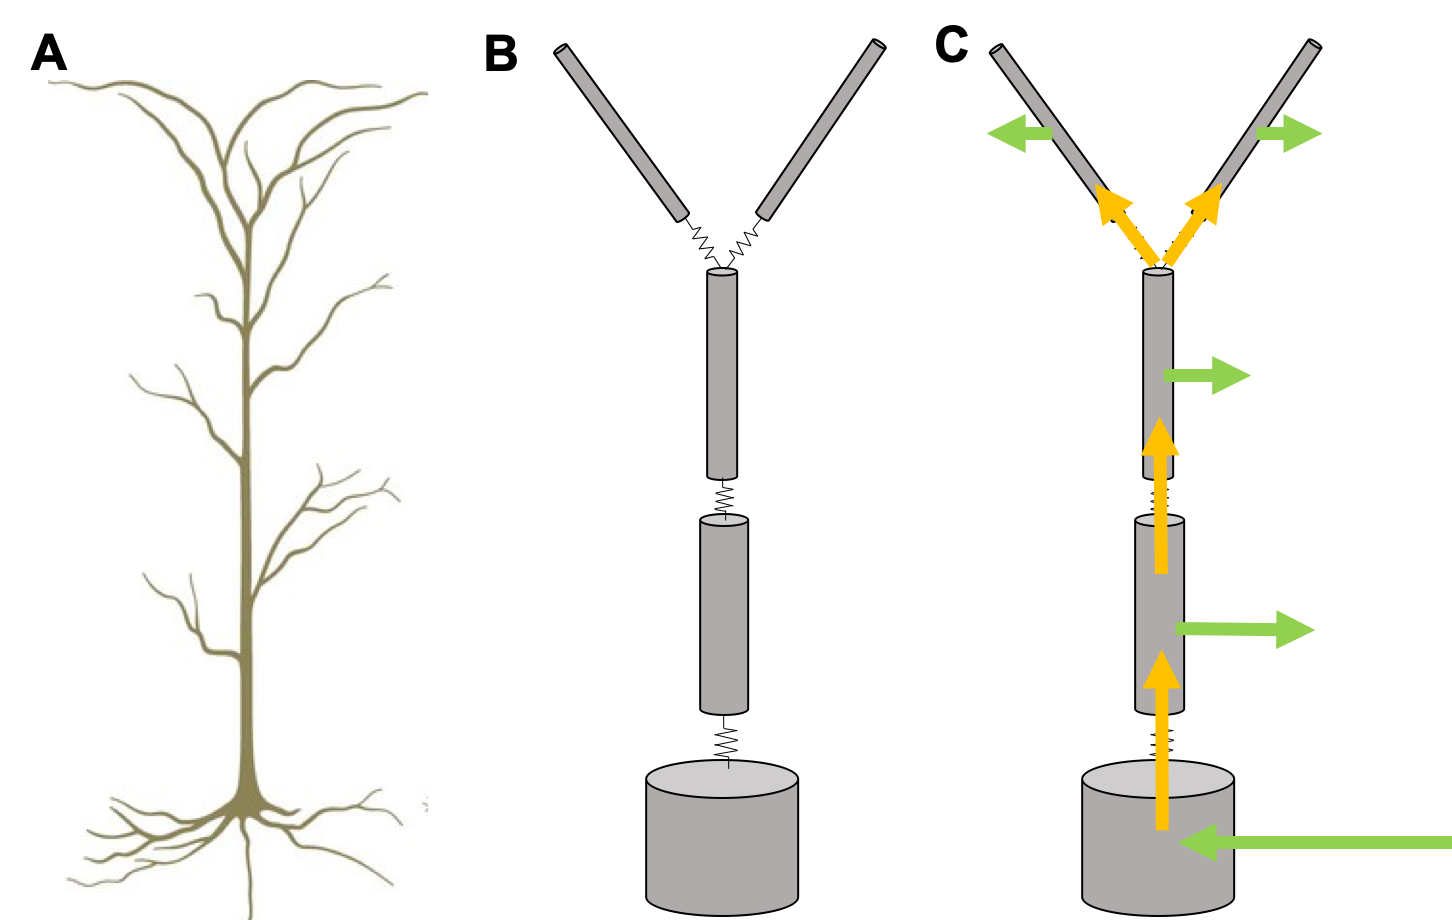
\includegraphics[width=0.6\textwidth]{Fig02/Multicomp.png}
\end{center}
\caption{\textbf{Multicompartmental modelling.} 
}
\label{fig:multicomp}
\end{figure}

Below, we first present a framework for modeling the transmembrane currents in a single compartment (subchapter called "Membrane currents"), and next show how a number of such compartments can be connected together to a multicompartment model (subchapter called "Morphology").


\subsection{Membrane currents}
In models based on a Hodgkin-Huxley type formalism, a patch of membrane typically includes three autonomous types of transmembrane currents. These are (i) a capacitive current density ($i_c$), (ii) a the leakage current density ($i_L$), and (iii) a the current density through various active ion channels ($i_x$), of which there can be several different kinds ($x$ is an index). In addition, a neuron may receive external stimuli, either through (iv) synaptic currents ($i_{syn}$) or (v) experimental current injections ($i_{stim}$). In the case where the neuron is modeled as a single compartment, the net transmembrane current must be zero, so that:

\begin{equation}
i_c + i_L + \sum_x{i_x} + i_{syn} + i_{stim} = 0.
\label{eq:singlecomp_zerosum}
\end{equation}
Below, we define the various currents that go into this equation.

\subsubsection{Capacitive current}
The capacitive current, 
\begin{equation}
i_c = c_m \frac{d\phi_m}{dt},
\label{eq:HHcap}
\end{equation}
represents the charging up of the membrane potential $\phi_m$ due to a charge density accumulating on the outside of inside of the capacitive membrane. Here, $c_m$ is the specific membrane capacitance. In the HH-model, $c_m$ had the value
1 $\mu$F/cm$^2$, and this value seems to be representative for most neurons.  An illustration of how to interpret the capacitive current is given in Fig. \ref{fig:capacitive_currents}. 

\begin{figure}[!ht]
\begin{center}
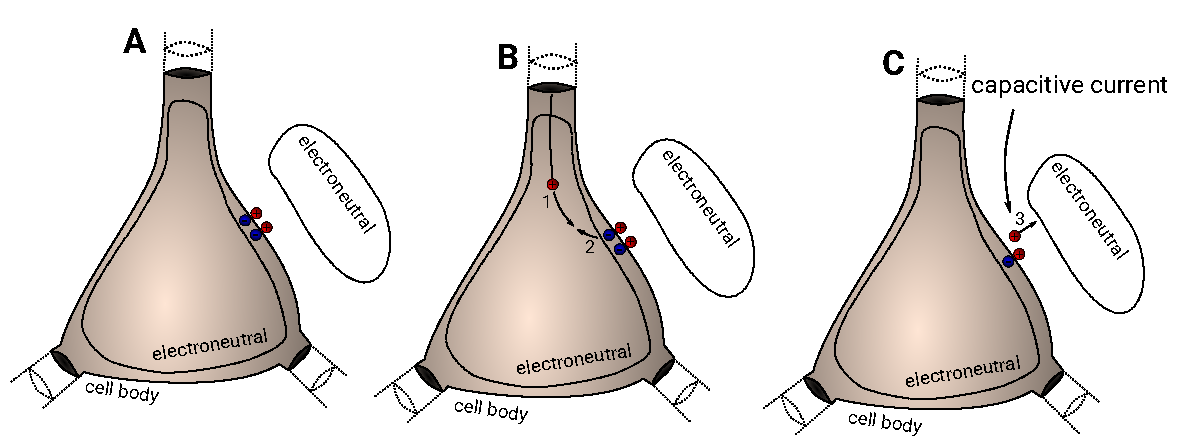
\includegraphics[width=0.8\textwidth]{Fig02/capacitive_currents.pdf}
\end{center}
\caption{\textbf{Capacitive currents are important for current conservation.}  (\textbf{(A)}) The extracellular and intracellular bulk solutions are essentially electroneutral, and the only region where there is a nonzero charge density is in the thin debye layers around the capacitive membrane. The capacitive current is not due to ions crossing the membrane, but due to ions piling up on either side of it, separating a charge density $\rho$ and a charge density $-\rho$, giving rise to a membrane potential of $\phi_m = \rho/c_m$. An outward capacitive current could correspond to an anion leaving the membrane on the inside (\textbf{(B)}), which will coincide with a cation leaving the membrane on the outside (\textbf{(C)}). Thus, capacitive membrane currents give rise to electrical ionic volume currents both in the intra- and extracellular space. 
}
\label{fig:capacitive_currents}
\end{figure}


\subsubsection{Leakage current}
The leakage current is expressed as
\begin{equation}
i_L = \bar{g}_L (\phi_m - E_L),
\label{eq:HHleak}
\end{equation}
where $\bar{g}_L$ is the leak conductance (the bar indicates that it's a constant). The factor $(\phi_m - E_L)$ is often called the driving force, and $E_L$ is the leak reversal potential. The biophysical origin of the reversal potential is explained later (see SECTION). For now, we will simply think of $E_L$ as a constant, and the leakage current as representative of an orchestra of physiological processes that together will drive the membrane potential towards this constant value. Together, the capacitive current and the leakage current form an RC-circuit that determines the passive properties of the membrane. If the neuron were to include only these two currents, it could be well modelled as an RC-circuit (Fig. \ref{fig:RC}). Such RC-neuron models are often used to simulate the subthreshold dynamics of neurons.

\begin{figure}[!ht]
\begin{center}
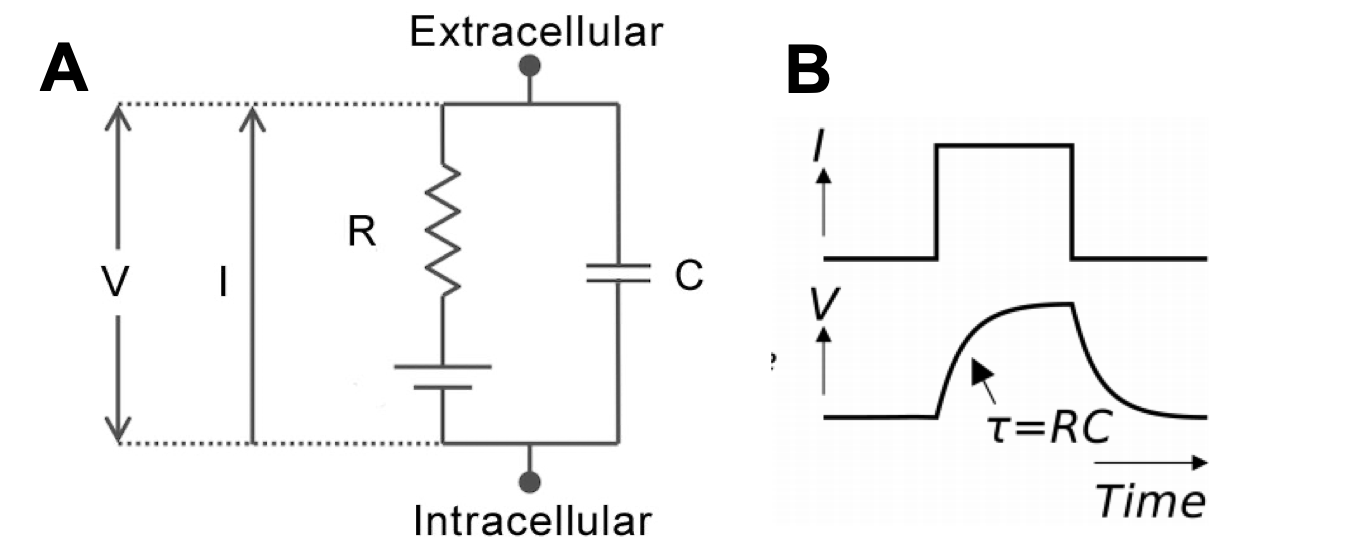
\includegraphics[width=0.8\textwidth]{Fig02/RCneuron.png}
\end{center}
\caption{\textbf{RC-neuron.}  A neuron model containing only a capacitive and a leakage current can be represented as an RC-circuit ($R = 1/g_L$). In the illustration, the neuron is given a current injection $I$ and responds by charging up the membrane. When the input is terminated, the membrane potential will return to the value $E_L$.
}
\label{fig:RC}
\end{figure}

In the RC-model, $E_L$ will be identical to the resting potential of the neuron. In the more general models, which also include active ion channels (see below), the resting potential will still tend to be close to $E_L$, but will typically not be identical to $E_L$, as there some of the active ion channels can be partially open during rest. In the HH model, $E_L$ had the value $-54.4$ mV. 


\subsubsection{Active ion channels}
In addition to $I_c$ and $I_L$, biophysical neuronal models typically include a number of active ion channels. When based on a Hodgkin-Huxley type formalism, current through an active an active ion channel $x$ is modeled as:

\begin{equation}
I_x = \bar{g}_x m_x^{\alpha} h_x^{\beta}(V-E_x)
\label{eq:HHform}
\end{equation}

Here, $\bar{g}_x$ denotes the conductance all channels of type $x$ are fully open (the bar indicates that it's a constant), while $E_x$ is the reversal potential for the ion species that travels through the channel.

An active ion channel differs from the passive leakage channel in that its total conductance, $\bar{g}_{x} m^{\alpha} h^{\beta}$, will vary with time due to the so-called gating variables, $m$ and $h$, which determine the dynamics of how the ion channel activates or deactivates (opens or closes). Here, $m$ and $h$ represent two different types of gates, which have different dependencies in terms of when they open/close. The exponents $\alpha$ and $\beta$ indicate that a channel $x$ may have several copies of each type of gate.  At the cellular level, the values of $m$ and $h$ interpret as the fraction of the gates of the various types that are open, and the values are thus numbers between zero (all gates in the closed state) and one (all gates in the open state). For an ion channel to be open, all its gates must be in the open state. The product $m^{\alpha} h^{\beta}$ thus interprets as the fractions of ion channels that are open.

For voltage-gated ion channels, the the dynamics of the gating variables are described by kinetics equations on the form:
\begin{equation}
\frac{dx(\phi_m,t)}{dt} = \frac{x_{\infty}(\phi_m) - x}{\tau_x(\phi_m}),  \, \text{for } x = \{m,h\}.
\label{eq:HHgate}
\end{equation}
The same kind of formalism also applies to ligand gated ion channels, i.e., channels that instead of opening and closing as a function of the membrane potential $\phi_m$, open or close as a function of a concentration of some ligand. The most common ligand gated channels in the brain are Ca$^{2+}$ gated ion channels. Here, the steady state activation $x_{inflty}(\phi_m)$ and activation time constant $\tau_x(\phi_m)$ are functions of the membrane potential, and these must be determined experimentally for each individual ion channel type. We do not go into these experimental issues here. 



and  $\bar{g}_{K} n^4$ are functions of voltage and time via the so-called gating variables $m$, $h$ and $n$. The exponents indicate that the Na$^+$ channels has three copies of a gate of type $m$, and one copy of a gate of type $h$, while the K$^+$ has only one kind of gate, but four copies of it. At the cellular level, $m$, $h$ and $n$ interpret as the fraction of the the gates that are open, and they thus take numbers between zero (all gates in the closed state) and one (all gates in the open state). The products $m^3 h$ and $n^4$ thus interpret as the fractions of the Na$^+$ channels and the K$^+$ channels that are open, respectively. The dynamics of the gating variables are described by kinetics equations on the form:


the original HH model contains two active ion channels, a Na$^+$ and a K$^+$ channel, which together are responsible for action potential generation:
\begin{equation}
i_{Na} = \bar{g}_{Na} m^3 h (\phi_m - E_{Na}),
\label{eq:HHNa}
\end{equation}
\begin{equation}
i_{K} = \bar{g}_{K} n^4 (\phi_m - E_{K}).
\label{eq:HHK}
\end{equation}
Here, $\bar{g}_{Na}$ and $\bar{g}_K$ are the conductances for fully open channels (the bars indicate that they are constants), while $E_{Na}$ and $E_{K}$ are the Na$^+$ and K$^+$ reversal potentials, which in the HH model had the values $50$ mV and $-77$ mV, respectively. Like the leakage current will tend to drive $\phi_m$ towards $E_L$, the Na$^+$ current, when active, will tend to drive $\phi_m$ towards $E_{Na}$, and the K$^+$ current will tend to drive $\phi_m$ towards $E_K$. 

The active channels differ from the passive leakage channel in that their total conductances $\bar{g}_{Na} m^3 h$ and  $\bar{g}_{K} n^4$ are functions of voltage and time via the so-called gating variables $m$, $h$ and $n$. The exponents indicate that the Na$^+$ channels has three copies of a gate of type $m$, and one copy of a gate of type $h$, while the K$^+$ has only one kind of gate, but four copies of it. At the cellular level, $m$, $h$ and $n$ interpret as the fraction of the the gates that are open, and they thus take numbers between zero (all gates in the closed state) and one (all gates in the open state). The products $m^3 h$ and $n^4$ thus interpret as the fractions of the Na$^+$ channels and the K$^+$ channels that are open, respectively. The dynamics of the gating variables are described by kinetics equations on the form:
\begin{equation}
\frac{dx(\phi_m,t)}{dt} = \frac{x_{\infty}(\phi_m) - x}{\tau_x(\phi_m}),  \, \text{for } x = \{m,n,h\}.
\label{eq:HHgate}
\end{equation}
Here, the steady state activation $x_{inflty}(\phi_m)$ and activation time constant $\tau_x(\phi_m)$ are functions of the membrane potential which must be determined experimentally. This is quite some work, and we do not go into these experimental issues here. 

In the original study by Hodgkin and Huxley it was found that:
\begin{equation}
x_{\infty}(\phi_m) = \frac{\alpha_x(\phi_m)}{\alpha_x(\phi_m) + \beta_x(\phi_m)}, 
\label{eq:xinfly}
\end{equation}
and
\begin{equation}
\tau_{x}(\phi_m) = \frac{1}{\alpha_x(\phi_m) + \beta_x(\phi_m)}, 
\label{eq:taux}
\end{equation}
with
\begin{eqnarray}
\alpha_n = 0.01 \frac{\phi_m+55}{1-e^{-(\phi_m+55)/10}}, \\
\beta_n = 0.125 e^{-(\phi_m+65)/80}, \\
\alpha_m = 0.1 \frac{\phi_m+40}{1-e^{-(\phi_m+40)/10}}, \\
\beta_m = 4 e^{-(\phi_m+65)/18}, \\
\alpha_h = 0.07 e^{-(\phi_m+65)/20}, \\
\beta_h = \frac{1}{1+e^{-(\phi_m+35)/10}}, 
\end{eqnarray}
where $\phi_m$ should be inserted with units mV for things to become correct. 


\subsubsection{Active ion channels in Hodgkin-Huxley type models}
The Hodgkin-Huxley model was adapted to experiments performed on the giant axon in a motor neuron of a squid. The reason for this was simply that this kind of neuron was very large, which made it easy to record from and manipulate experimentally. In general, neurons come in many varieties, and their dynamical properties vary. The Hodgkin-Huxley model is limited in its ability to capture the dynamics of, say, a pyramidal cell in the mammalian cortex. Fortunately, however, the type of mathematical formalism used to describe the ion channel dynamics is still applicable to most neuronal mechanisms. 

In models based on a Hodgkin-Huxley type formalism, a patch of membrane typically include three various types of transmembrane currents. These are (i) a capacitive current density ($i_c$), (ii) a the leakage current density ($i_L$), and (iii) a the current density through active ion channels ($i_x$), of which there can be several different kinds ($x$ is an index). 





ion channels are described on the equational form

\begin{equation}
I_x = g_x m_x^{\alpha} h_x^{\beta}(V-E_x)
\label{eq:HHform}
\end{equation}


\begin{figure}[!ht]
\begin{center}
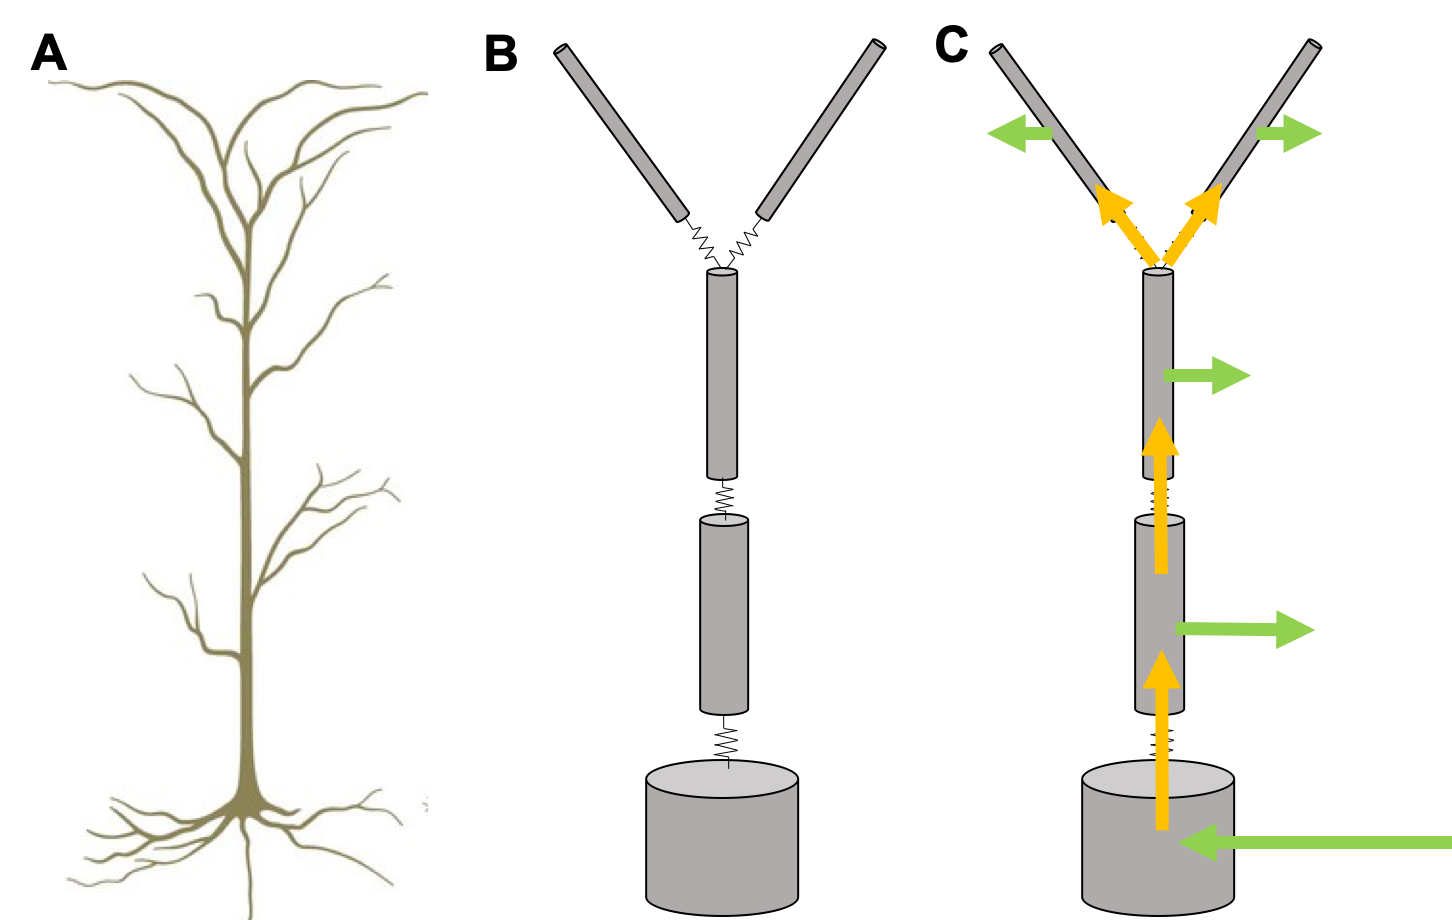
\includegraphics[width=0.6\textwidth]{Fig02/Multicomp.png}
\end{center}
\caption{\textbf{Multicompartmental modelling.} 
}
\label{fig:multicomp}
\end{figure}



\subsubsection{Morphology}
\ghnote{Skriv om multicomp her}

\subsection{Cable theory}
\ghnote{Skriv om cable theory her, og noen analytiske tilfeller som hjelper oss aa faa en kjerneforstaaelse.}




\subsection{Point neurons}
\ghnote{skriv om punktmodeller her, problemet med at de ikke gir opphav til ekstracellulare felter, og triks for aa bruke dem likevel.}
\tvnnote{Gir det egentlig mening å gå inn på dette før vi har introdusert VC-teori? Hva med å bare kort gå via punktnevroner i utledningen av kabel-ligningen, og henvise til senere seksjoner?}
\subsection{Constant concentrations approximation}
\ghnote{Skrive om konsentrasjonseffekter. Tror det er bra aa spare Nernst-potensialene til dette delkap. Si noe om at man ofte ikke trenger aa holde styr paa konsentrasjoner pga. homeostatiske mekanismer "bakt inn" i passiv lekkasje.Si noe om hva som skal til for faktisk aa modellere konsentrasjoner uten aa gaa inn i detalj. Referere til rammeverkene som kommer i Kap 6.}
